% signed-tropical.tex — publication-grade figure of lling-llang's signed-tropical
% semiring (ℝ∪{±∞}, min, +, +∞, 0): the full real line so rewards are negative costs.
% Shows the cost/neutral/reward number line and the star-convergence boundary at 0.
% Native ⊕/⊗/0̄/1̄ typography. Palette: docs/diagrams/README.md.
% Compile: lualatex --output-format=dvi signed-tropical.tex ; dvisvgm --no-fonts signed-tropical.dvi
\documentclass[dvisvgm,border=6pt]{standalone}
\usepackage{fontspec}
\usepackage{amsmath,amssymb}
\usepackage{tikz}
\usetikzlibrary{positioning,fit,backgrounds,arrows.meta,decorations.pathreplacing}

% palette (docs/diagrams/README.md)
\definecolor{foundation}{HTML}{BBDEFB}\definecolor{foundationB}{HTML}{1565C0}
\definecolor{algorithms}{HTML}{C8E6C9}\definecolor{algorithmsB}{HTML}{2E7D32}
\definecolor{speech}{HTML}{FFE0B2}\definecolor{speechB}{HTML}{E65100}
\definecolor{verify}{HTML}{FFCDD2}\definecolor{verifyB}{HTML}{B71C1C}
\definecolor{ink}{HTML}{102027}\definecolor{edge}{HTML}{607D8B}

\begin{document}
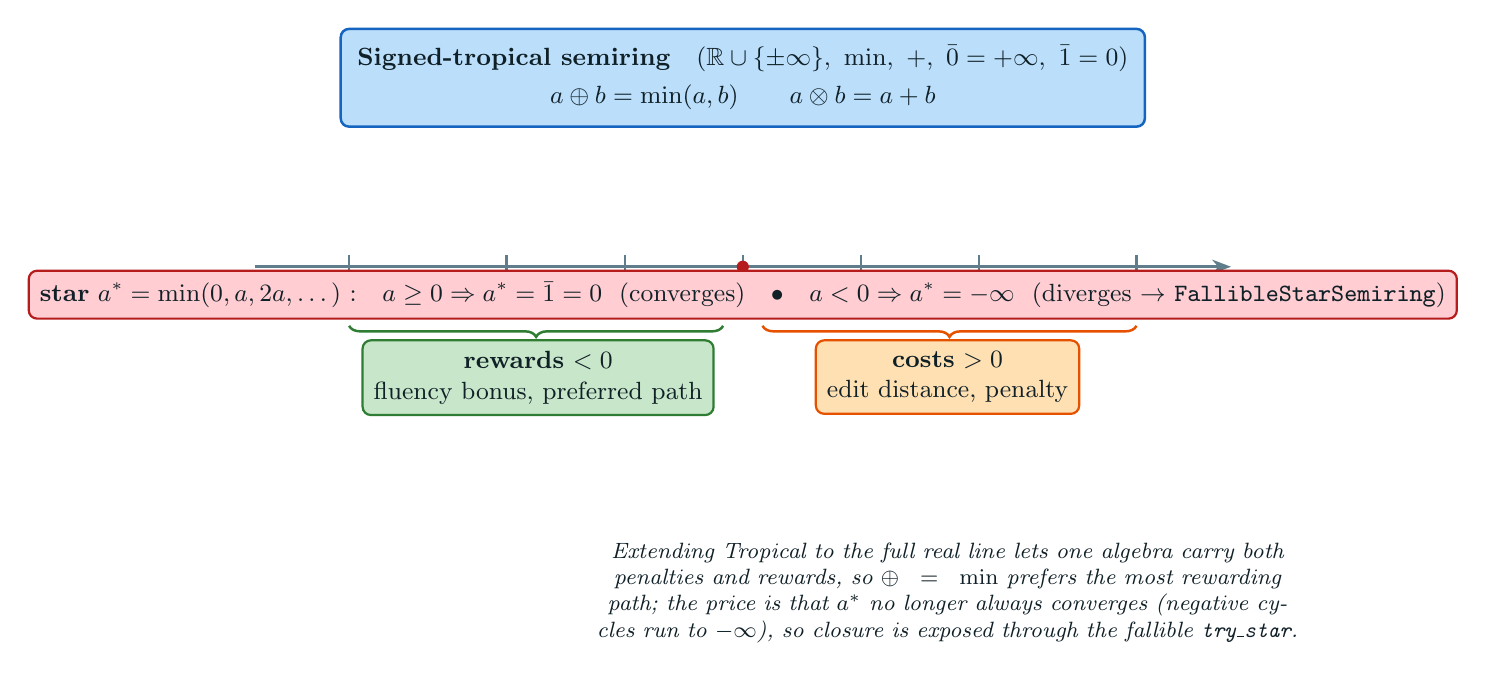
\begin{tikzpicture}[
    every node/.style={font=\small, text=ink},
    sig/.style={draw=foundationB, fill=foundation, rounded corners=3pt, align=center,
                inner sep=6pt, line width=0.9pt},
    rewardbox/.style={draw=algorithmsB, fill=algorithms, rounded corners=3pt, align=center,
                      inner sep=4pt, line width=0.8pt},
    costbox/.style={draw=speechB, fill=speech, rounded corners=3pt, align=center,
                    inner sep=4pt, line width=0.8pt},
    divbox/.style={draw=verifyB, fill=verify, rounded corners=3pt, align=center,
                   inner sep=4pt, line width=0.8pt},
    rel/.style={-{Stealth[length=2.4mm]}, draw=edge, line width=0.9pt},
  ]

  % the signature, at the top
  \node[sig] (sig) {\textbf{Signed-tropical semiring}\quad
        $(\mathbb{R}\cup\{\pm\infty\},\ \min,\ +,\ \bar 0={+}\infty,\ \bar 1=0)$\\[3pt]
        $a \oplus b = \min(a,b)\qquad a \otimes b = a + b$};

  % the number line
  \coordinate (L) at (-6.2,-2.4);
  \coordinate (R) at ( 6.2,-2.4);
  \draw[rel, line width=1.0pt] (L) -- (R);

  % tick marks and labels at -2,-1,0,1,2 and ±∞ ends
  \foreach \x/\lab in {-5/{$-\infty$}, -3/{$-2$}, -1.5/{$-1$}, 0/{$0=\bar 1$}, 1.5/{$1$}, 3/{$2$}, 5/{$+\infty=\bar 0$}} {
    \draw[edge, line width=0.8pt] (\x,-2.25) -- (\x,-2.55);
    \node[font=\footnotesize, below] at (\x,-2.55) {\lab};
  }

  % reward region (negative): green brace below-left
  \draw[decorate, decoration={brace, amplitude=4pt, mirror}, draw=algorithmsB, line width=0.9pt]
        (-5,-3.15) -- (-0.25,-3.15);
  \node[rewardbox, below=2pt of {(-2.6,-3.25)}] (rew)
        {\textbf{rewards} $<0$\\ fluency bonus, preferred path};

  % cost region (positive): orange brace below-right
  \draw[decorate, decoration={brace, amplitude=4pt, mirror}, draw=speechB, line width=0.9pt]
        (0.25,-3.15) -- (5,-3.15);
  \node[costbox, below=2pt of {(2.6,-3.25)}] (cst)
        {\textbf{costs} $>0$\\ edit distance, penalty};

  % star convergence boundary marker at 0
  \fill[verifyB] (0,-2.4) circle (2.2pt);

  % explicit star-rule annotations
  \node[divbox, below=20mm of sig, xshift=0mm, yshift=2mm] (starrule)
        {\textbf{star} $a^{*}=\min(0,a,2a,\dots)$\ :\quad
         $a\ge 0 \Rightarrow a^{*}=\bar 1=0$ \ (converges)\quad$\bullet$\quad
         $a<0 \Rightarrow a^{*}=-\infty$ \ (diverges $\to$ \texttt{FallibleStarSemiring})};

  % caption
  \node[below=15mm of cst.south, xshift=-0mm, text width=112mm, align=center,
        font=\footnotesize\itshape]
        {Extending Tropical to the full real line lets one algebra carry both penalties
         and rewards, so $\oplus=\min$ prefers the most rewarding path; the price is that
         $a^{*}$ no longer always converges (negative cycles run to $-\infty$), so closure
         is exposed through the fallible \texttt{try\_star}.};
\end{tikzpicture}
\end{document}
